%! TeX program = lualatex
\documentclass[a4paper]{article} 

\usepackage[backend=biber, style=numeric, date=iso, urldate=iso]{biblatex}
\addbibresource{references.bib}
\DeclareFieldFormat{urldate}{Accessed on: #1}
\usepackage{amsmath}
% packages
\usepackage{microtype}      % Slightly tweak font spacing for aesthetics
\usepackage[english]{babel} % Language hyphenation and typographical rules
\usepackage[final, colorlinks = true, urlcolor = black, linkcolor = black, citecolor = black]{hyperref} 
\usepackage{changepage}     % adjust margins on the fly

\usepackage{fontspec}
\setmainfont{EB Garamond}
\setmonofont[Scale=MatchLowercase]{Deja Vu Sans Mono}

\usepackage{minted}
\usemintedstyle{algol_nu}
\usepackage{xcolor}

\usepackage{pgfplots}
\pgfplotsset{width=\textwidth,compat=1.9}

\usepackage{caption}
\newenvironment{code}{\captionsetup{type=listing}}{}
\captionsetup[listing]{skip=0pt}
\setlength{\abovecaptionskip}{5pt}
\setlength{\belowcaptionskip}{5pt}

\usepackage[yyyymmdd]{datetime}
\renewcommand{\dateseparator}{--}

\usepackage{titlesec}
% \titleformat{\section}{\LARGE\bfseries}{}{}{}[\titlerule]
% \titleformat{\subsection}{\Large\bfseries}{}{0em}{}
% \titlespacing{\subsection}{0em}{-0.7em}{0em}
%
% \titleformat{\subsubsection}{\large\bfseries}{}{0em}{$\bullet$ }
% \titlespacing{\subsubsection}{1em}{-0.7em}{0em}

% margins
\addtolength{\hoffset}{-2.25cm}
\addtolength{\textwidth}{4.5cm}
\addtolength{\voffset}{-3.25cm}
\addtolength{\textheight}{5cm}
\setlength{\parskip}{0pt}
\setlength{\parindent}{0in}
% \setcounter{secnumdepth}{0}

\begin{document}
\hrule \medskip
\begin{minipage}{0.295\textwidth} 
    \raggedright
    \footnotesize 
    \begin{tabular}{@{}l l}
        Name: & Andrew Hayes \\
        Student ID: & 21321503 \\
        E-mail: & \href{mailto://a.hayes18@universityofgalway.ie}{\texttt{a.hayes18@universityofgalway.ie}} \\
    \end{tabular}
\end{minipage}
\begin{minipage}{0.4\textwidth} 
    \centering 
    \vspace{0.4em}
    \LARGE
    \textsc{ct421} \\ 
\end{minipage}
\begin{minipage}{0.295\textwidth} 
    \raggedleft
    \today
\end{minipage}
\medskip\hrule 
\begin{center}
    \normalsize
    Project 1: Evolutionary Search
\end{center}
\hrule
\medskip

\section{Implementation \& Design}
I chose to write my implementation of the evolutionary search algorithm in Python for ease \& speed of writing, and because Python has a number of libraries for mathematics \& machine learning that I could utilise to create an efficient solution.
I wrote two separate scripts: one named \verb|salesman.py| for the core implementation of the genetic algorithm which produces a tab-separated value (TSV) file of containing the results from each generation of the search and one named \verb|plots.py| to ingest these TSV files and plot the fitness over generations.
I decided to separate these functionalities into different scripts so that I could easily run the genetic algorithm without bothering to plot results during debugging \& testing, and so that results would only be plotted when necessary.

\subsection{Arguments}
The script accepts a large number of command-line arguments \& flags to control how the search is conducted.
Most of these are optional overrides for default values in the program.
The flags \& arguments accepted are:
\begin{itemize}
    \item   \verb|-h|, \verb|--help|: a flag to make the script output the possible flags \& command-line arguments that it accepts, and what they do.

    \item   \verb|-i|, \verb|--input-file INPUT_FILE|: the path to the input file in TSP format.
            The only mandatory argument that must be supplied to the script for it to run.

    \item   \verb|-s|, \verb|--size SIZE|: the population size of solutions to be initialised and used in each generation.
            This should be an integer value in the range $[1, \infty]$.

    \item   \verb|-g|, \verb|--num-generations NUM_GENERATIONS|: the number of generations the genetic algorithm should evolve over.
            This should be an integer value in the range $[1, \infty]$.

    \item   \verb|-a|, \verb|--give-up-after GIVE_UP_AFTER|: the number of generations to give up searching after if the best solution has remained unchanged for that number of generations.
            This allows the search to be prevented from going on too long after the possibility for improvement has been exhausted.
            This should be an integer value in the range $[1, \infty]$.

    \item   \verb|-p|, \verb|--selection-proportion SELECTION_PROPORTION|: the proportion of the population to be selected on each iteration and allowed to survive to the next generation.
            This should be a floating-point number in the range $[0, 1]$.

    \item   \verb|c|, \verb|--crossover-rate CROSSOVER_RATE|: the probability of a given pair of solution to sexually reproduce (crossover) and create offspring after surviving selection.
            Note that this is not the \textit{number} of solutions that will undergo crossover, as the number of solutions to undergo crossover is determined by the selection proportion and population size to maintain a constant population size; instead, candidate pairs for crossover are randomly selected and then that pair's probability of successfully producing offspring is determined by this value, and this continues until the required number of offspring are produced.
            This should be a floating-point number in the range $[0, 1]$.

    \item   \verb|-m|, \verb|--mutation-rate MUTATION_RATE|: like \verb|--crossover-rate|, this value determines the probability of a solution produced via crossover in that generation of undergoing mutation.
            Each child solution is iterated over, and has a chance of being mutated in accordance with this value.
            This should be a floating-point number in the range $[0, 1]$.

    \item   \verb|-o|, \verb|--output-file OUTPUT_FILE|: the path to the TSV file to which results should be outputted for a single run.

    \item   \verb|--quiet|: a flag to suppress output being printed.

    \item   \verb|--grid-search|: instead of just running the genetic algorithm once with some given parameters, iterate over a combination of population sizes, crossover rates, \& mutation rates to find the combination that yields the most fit solution.
            The values iterated over in the grid search are hard-coded into the Python script and can be changed only be editing the script, as manually typing out a list of parameters for each program run proved too cumbersome to be practical.
\end{itemize}

\subsection{Initialisation}
\subsubsection{TSP File Ingestion}
When the script is ran, the first function called is \mintinline{python}{graph_from_file(file)} which produces a Python dictionary object (essentially a hash map), containing the name of the TSP map in the file, the type, the comment, the dimension, the edge weight type, and a list of city dictionaries containing the name and $(x,y)$ co-ordinates of the city.
I couldn't easily find a formal specification of this file format online, so my parsing of these files assumes that certain values occur on certain lines and works for the three recommended files of \verb|berlin52.tsp|, \verb|kroA100.tsp|, \& \verb|pr1002.tsp|, but potentially could fail on more unusual TSP files.
(This is where I immediately regretted my choice of Python as a programming language when writing this function as this sort of thing is so much easier in Perl with its powerful regex engine).
\\\\
To avoid having to re-calculate the distances between cities every time I evaluated the fitness of a potential solution, I then run a function called \mintinline{python}{adjacency_matrix_from_graph(graph)} which returns an adjacency matrix (implemented as a two-dimensional list) where $A_{i,j}$ contains the distance between cities $i$ and $j$.
Here I made two further assumptions about the nature of the TSP files ingested:
\begin{itemize}
    \item   The function assumes that city names are an integer value in the range $[1, \infty]$ and thus the city $k$ is indexed at $k-1$.
    \item   The function also assumes that the TSP file's \verb|EDGE_WEIGHT_TYPE| is \verb|EUC_2D| and just calculates the two-dimensional Euclidean distance between the co-ordinates of the two cities.
\end{itemize}

\subsubsection{Population Initialisation}
To initialise the population, a function named \mintinline{python}{initialise_population(size, graph)} is ran which returns a list of random permutations of the ordered list of city names in the \mintinline{python}{graph} object.
Each random permutation will contain each city exactly once, and therefore the return to the start city is implied rather than outright represented in the list.
Then, a function called \texttt{list\_of\_fitnesses(population, adjacency\_matrix)} is ran which calculates the fitness of every tour in the population list and returns a list of fitnesses where the fitness at index $i$ is the fitness of the solution at index $i$ in the population.
This list is used to avoid re-calculating fitnesses unless absolutely necessary. 
The fitness is just the sum of the distances between each successive city in the tour, plus the distance between the final city and the start city to get the salesman back home.
\\\\
Then, a function named \mintinline{python}{get_current_best(population, fitnesses, generation)} is ran which finds the solution in the supplied population with the lowest corresponding fitness.
This function returns a dictionary containing the fittest tour in question, its fitness, and the generation in which it was found (set to \verb|0| in the initialisation stage).
Finally, the start time is saved as a UNIX timestamp and the output TSV data is initialised;
each line of TSV data is a string that is appended to a list of strings instead of one large string, as in Python string are immutable and each time a string is appended to, a new one is created, so it is more efficient to build up an array of strings.

\subsection{Evolution}
The evolution stage is a simple loop that iterates for the number of specified generations.

\subsubsection{Selection}
The first step performed in the evolution loop is selection.
I initially implemented this using Monte Carlo or Roulette Wheel selection, where each tour in the population is assigned a weight of $1 - \frac{\text{fitness}}{\text{total fitness}}$ where the total fitness is the sum of all fitnesses in the population.
Tours with higher weights were proportionally more likely to be selected to survive until the next generation.
I thought that this mode of selection would be good, as it means that even very weak solutions have a (small) chance of surviving and very good solutions have a (small) chance of dying: this theoretically helps prevent you getting stuck in local maxima by discarding weak solutions that contain a crucial component to the getting the optimal solution, and maintains diversity in the population.
However, when I ran the algorithm on \verb|berlin52.tsp| dataset with some arbitrary test parameters that I was using in the course of development, I got the following result:

\begin{figure}[H]
    \centering
    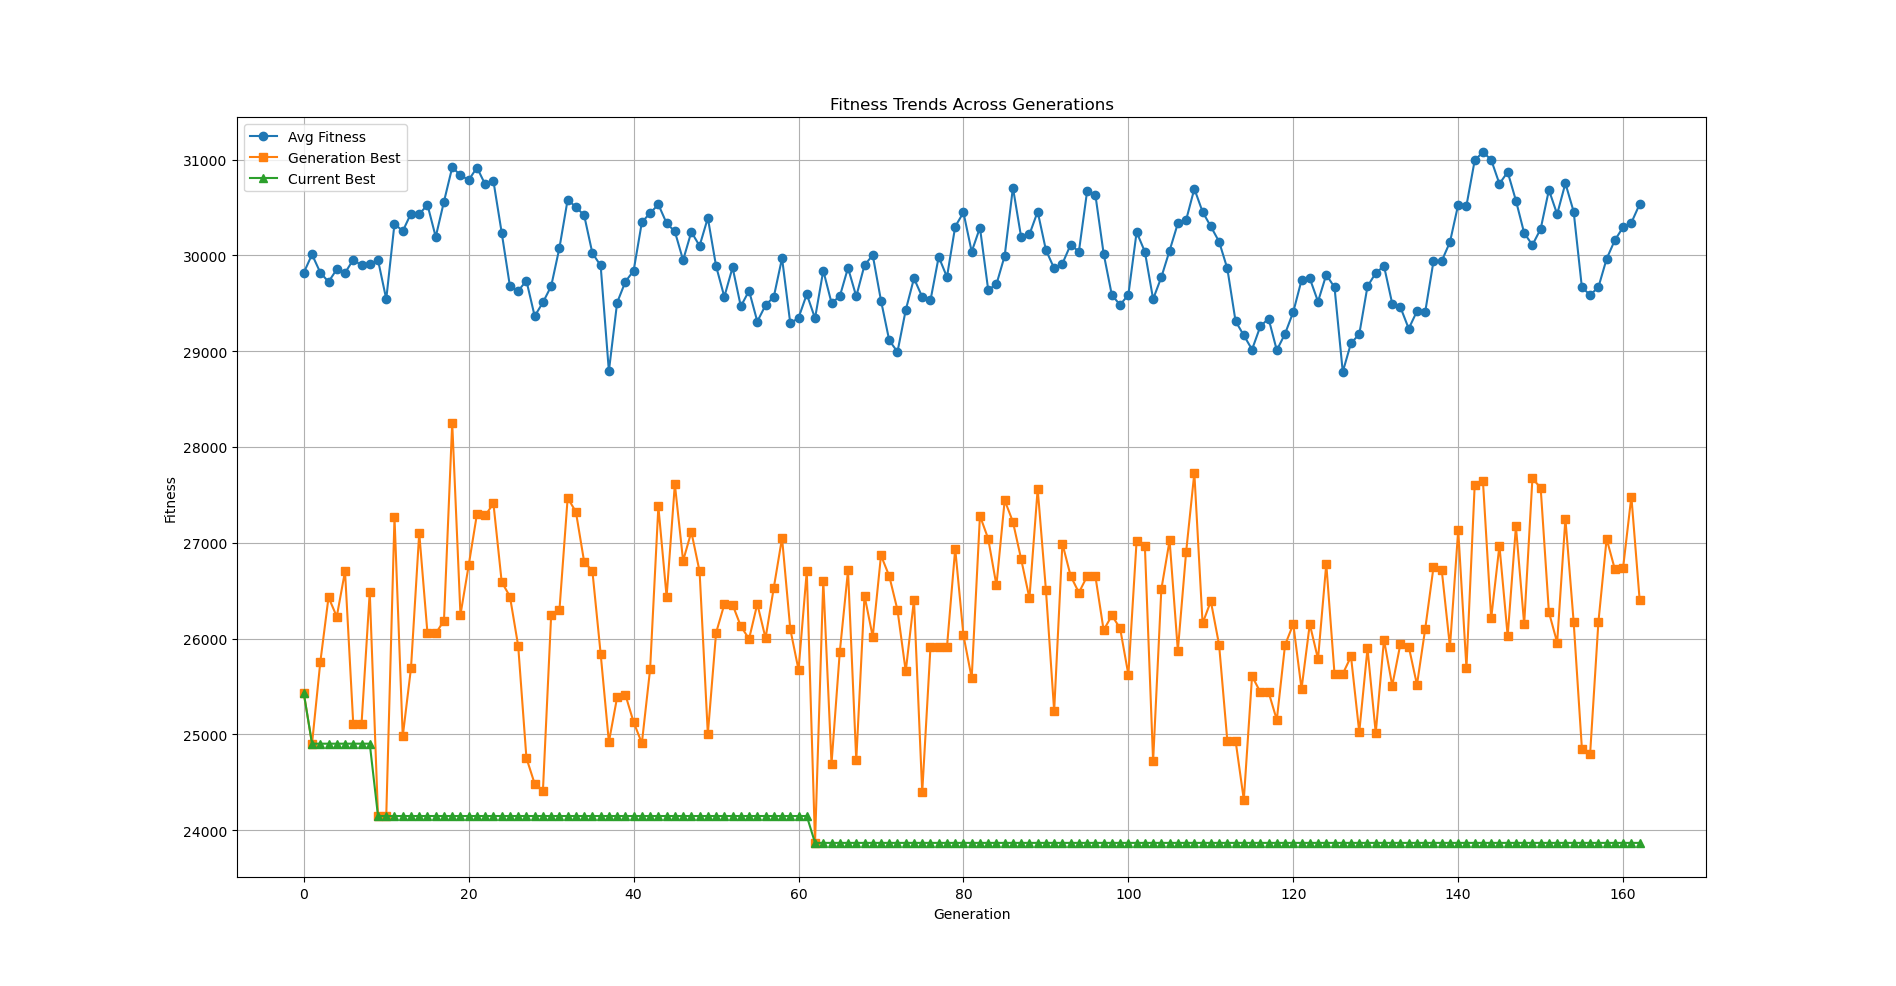
\includegraphics[width=\textwidth]{./images/berlin52_monte_defaults.png}
    \caption{Fitness over 200 generations for \texttt{berlin52.tsp} using Monte Carlo selection }
\end{figure}

As can be seen in the above figure, the algorithm didn't seem to be learning anything and, if anything, fitness seemed to be getting worse over generations.
Probably, the cause of this was that the weighting for Monte Carlo selection was not biased enough in favour of good solutions and against weak solutions, and it just resulted a fairly egalitarian deselection process which destroyed each generation's progress.
Any good solutions found from this process were more as a result of sheer luck than as a result of anything that can be described as learning or evolution.
I tried the same thing with a tournament selection process instead, and got the following results:

\begin{figure}[H]
    \centering
    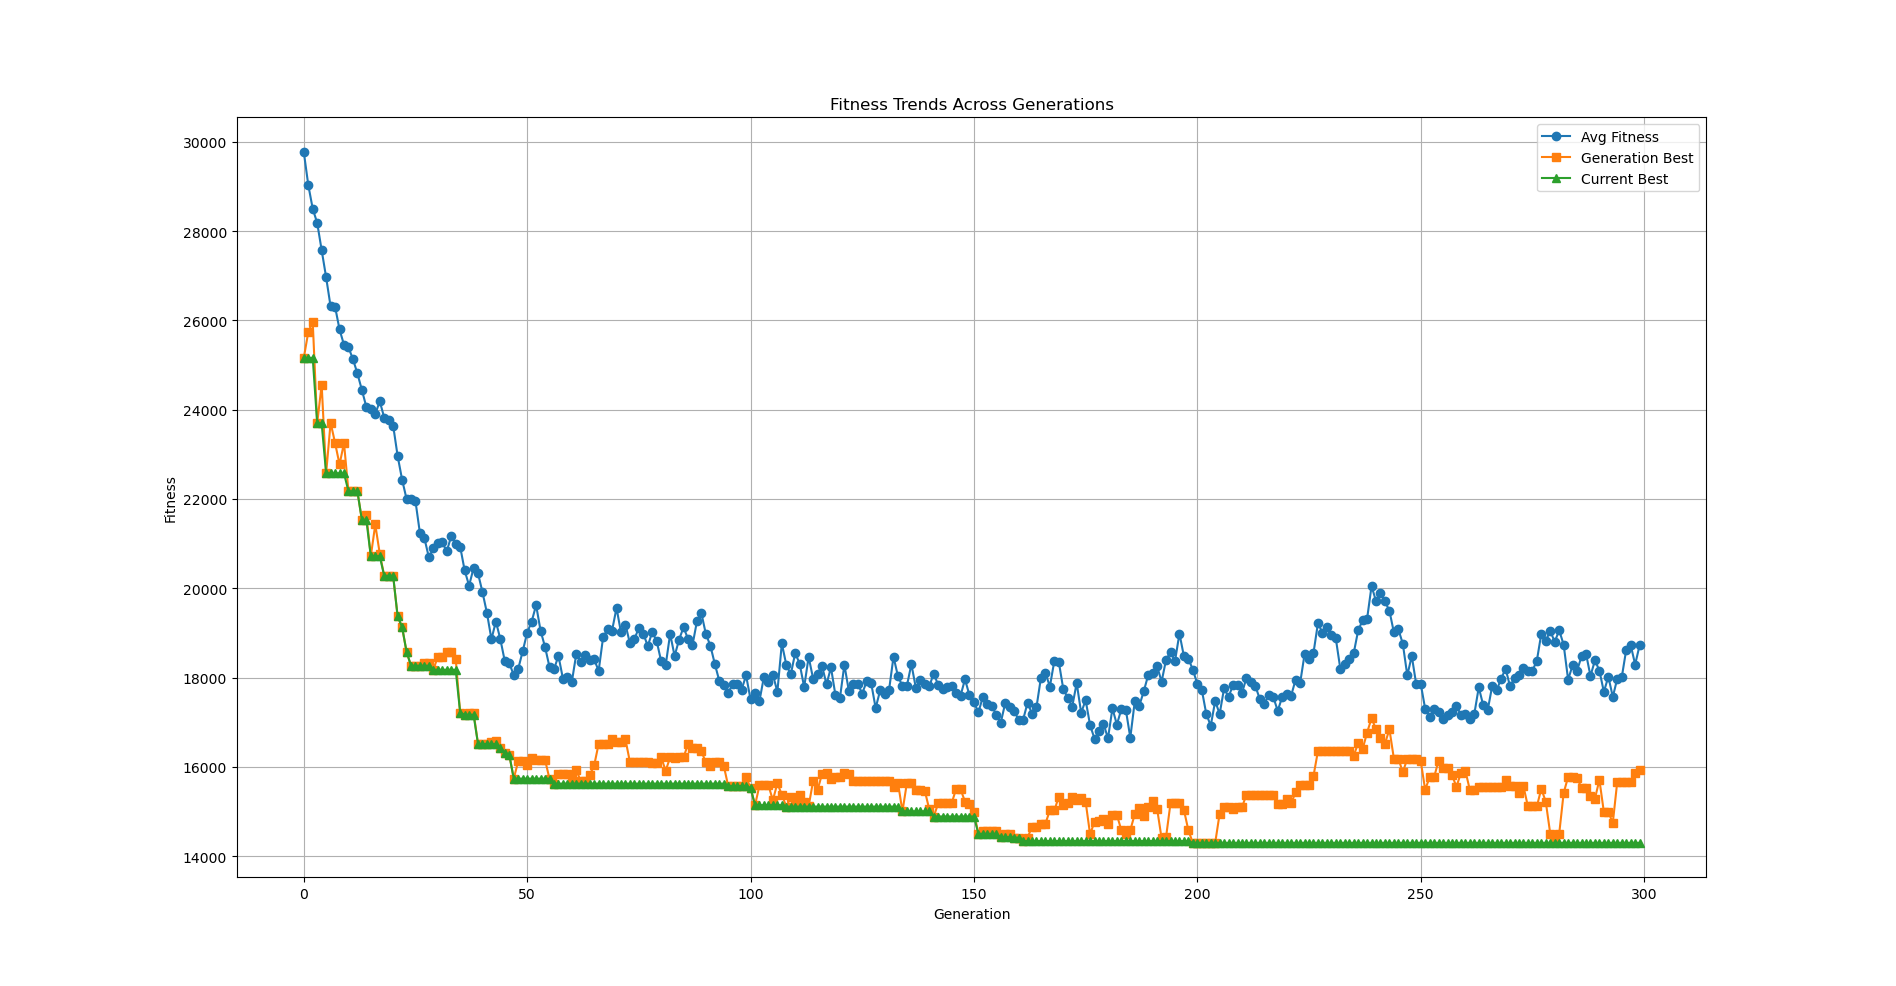
\includegraphics[width=\textwidth]{./images/berlin_52_tourn_defaults.png}
    \caption{Fitness over 200 generations for \texttt{berlin52.tsp} using tournament selection with a tournament size of 3}
\end{figure}

The difference in efficacy was so stark that I immediately abandoned using Monte Carlo selection in favour of tournament selection, although the failure of Monte Carlo selection here was more likely a result of poor implementation than as a result of genuine inappropriateness for the problem.
Tournament selection maintained the diversity I was looking for, giving an opportunity for survival to weaker solutions while maintaining a healthy population of increasingly fit solutions.

\subsubsection{Crossover}
Crossover is performed on the survivors of the selection process using a generalised \texttt{crossover(population, crossover\_rate, number\_to\_replace)} function which randomly alternates between Partially Mapped Crossover (PMX) and Order Crossover (OX), the algorithmic steps for which I took from Wikipedia\supercite{crossover}; while not a scholarly source for a reference, I feel that it's reasonable to use for the algorithmic steps in this case as they evidently produce the desired the results or do not and can be quite easily verified.
The generalised crossover function randomly alternated between the PMX and OX operators with equal probability.
\\\\
The PMX operator works as follows:
first, two indices within the two parent solutions are selected at random to serve as crossover points.
If the first crossover point occurs after second in the list, they are swapped.
Then, the sub-sequence from the first parent from the first crossover point to the second is copied directly to the child solution in the same positions.
Then, the second parent is iterated over from the first crossover point to the second crossover point:
for each city $m$ in the second parent that is not yet in the child solution, the city $n$ that occurs in the child at the index at which $m$ occurs in the parent is selected.
The index of $n$ in the second parent is found to create the partial mapping, and $m$ is copied into the child at the index at which $n$ occurs in the second parent, provided that index is empty in the child.
If the index occupied by $n$ in the parent is already occupied by some element $k$ in the child, $m$ is placed in the child at the index at which $k$ occurs in the second parent.
After the genes from the selected sub-sequence in the second parent are all copied into the child, the remaining positions in the child are filled with the genes from the second parent that still have yet to be copied into the child in the order that they appear in the second parent.
This is done by iterating over each index in the second parent, and if the city at that index is not found in the child, it is inserted into the child in the next empty position, until every city is accounted for and every index in the child is filled.
Thus, high-quality sub-sequences that have evolved in the parents have a chance of being preserved in the child, while introducing variance.
The partial mapping allows us to ensure that the child solution remains a valid solution with no duplication of cities.
\\\\
The OX operator works as follows:
like the PMX operator, two crossover points are selected at random and the sub-sequence defined by these crossover points is copied directly from the first parent into the child.
Then, each index in the second parent is iterated over, and if the city and that index in the second parent does not occur in the child, it is copied into the child into the first empty index after the second crossover point, wrapping around and starting from the 0\textsuperscript{th} index of the child once the end of the child list is reached.
The OX operator was chosen as it is slightly simpler than the PMX operator, preserving only the order of cities in the tour, rather than relative mappings, thus introducing more randomness into the child solution and therefore increasing the diversity of the gene pool.
However, during testing I came to realise that I tended to get better fitnesses using just the PMX operator and no OX, so I stopped using OX in the generalised crossover function and used only PMX.
During the course of development, I ran two test runs with my default, untuned parameters on the \verb|berlin52.tsp| dataset for the PMX-only crossover and the PMX+OX crossover.
PMX-only yielded a best fitness of 8207 while PMX+OX yielded a significantly worse best fitness of 13317.
The reason for this is probably that the OX operator was introducing too much randomness into the crossover and losing important mappings from the evolved solutions, this conjecture being supported by the fitness graphs for the two runs:

\begin{figure}[H]
    \centering
    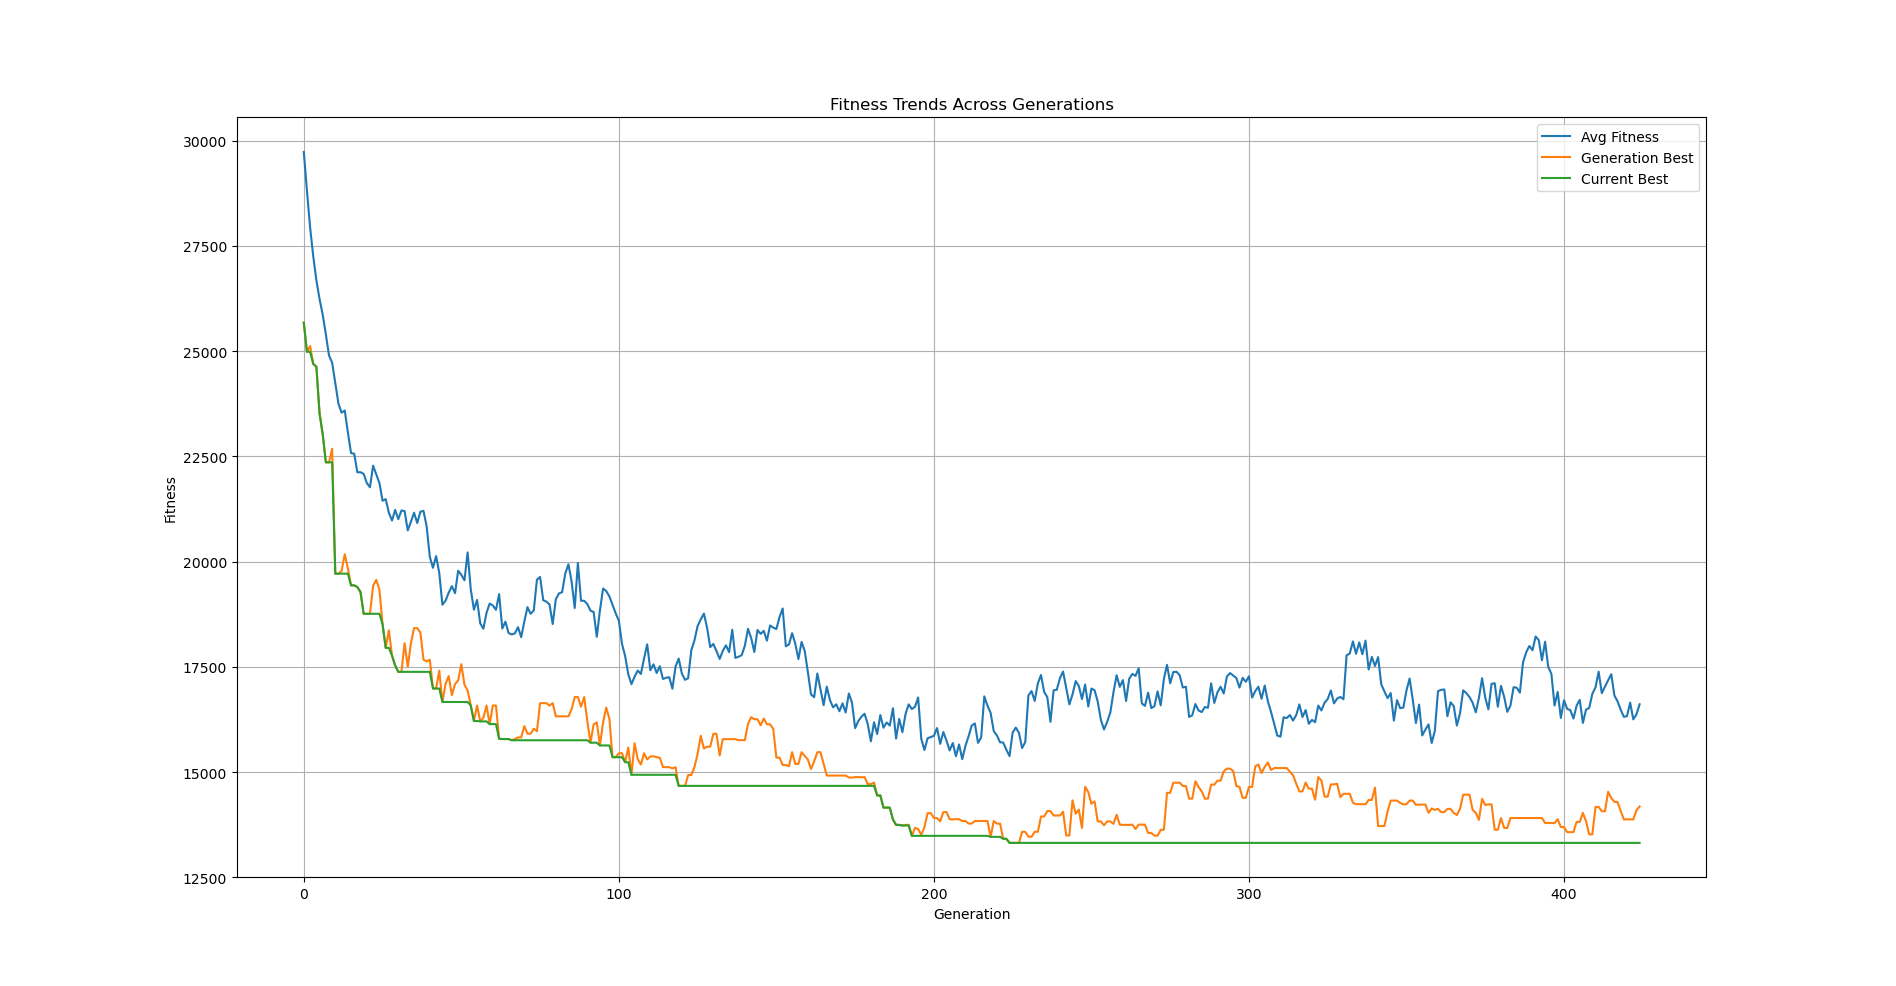
\includegraphics[width=\textwidth]{./images/berlin52_defaults_pmxox.png}
\caption{Fitness achieved with PMX+OX crossover on \texttt{berling52.tsp} using the default parameters}
\end{figure}

\begin{figure}[H]
    \centering
    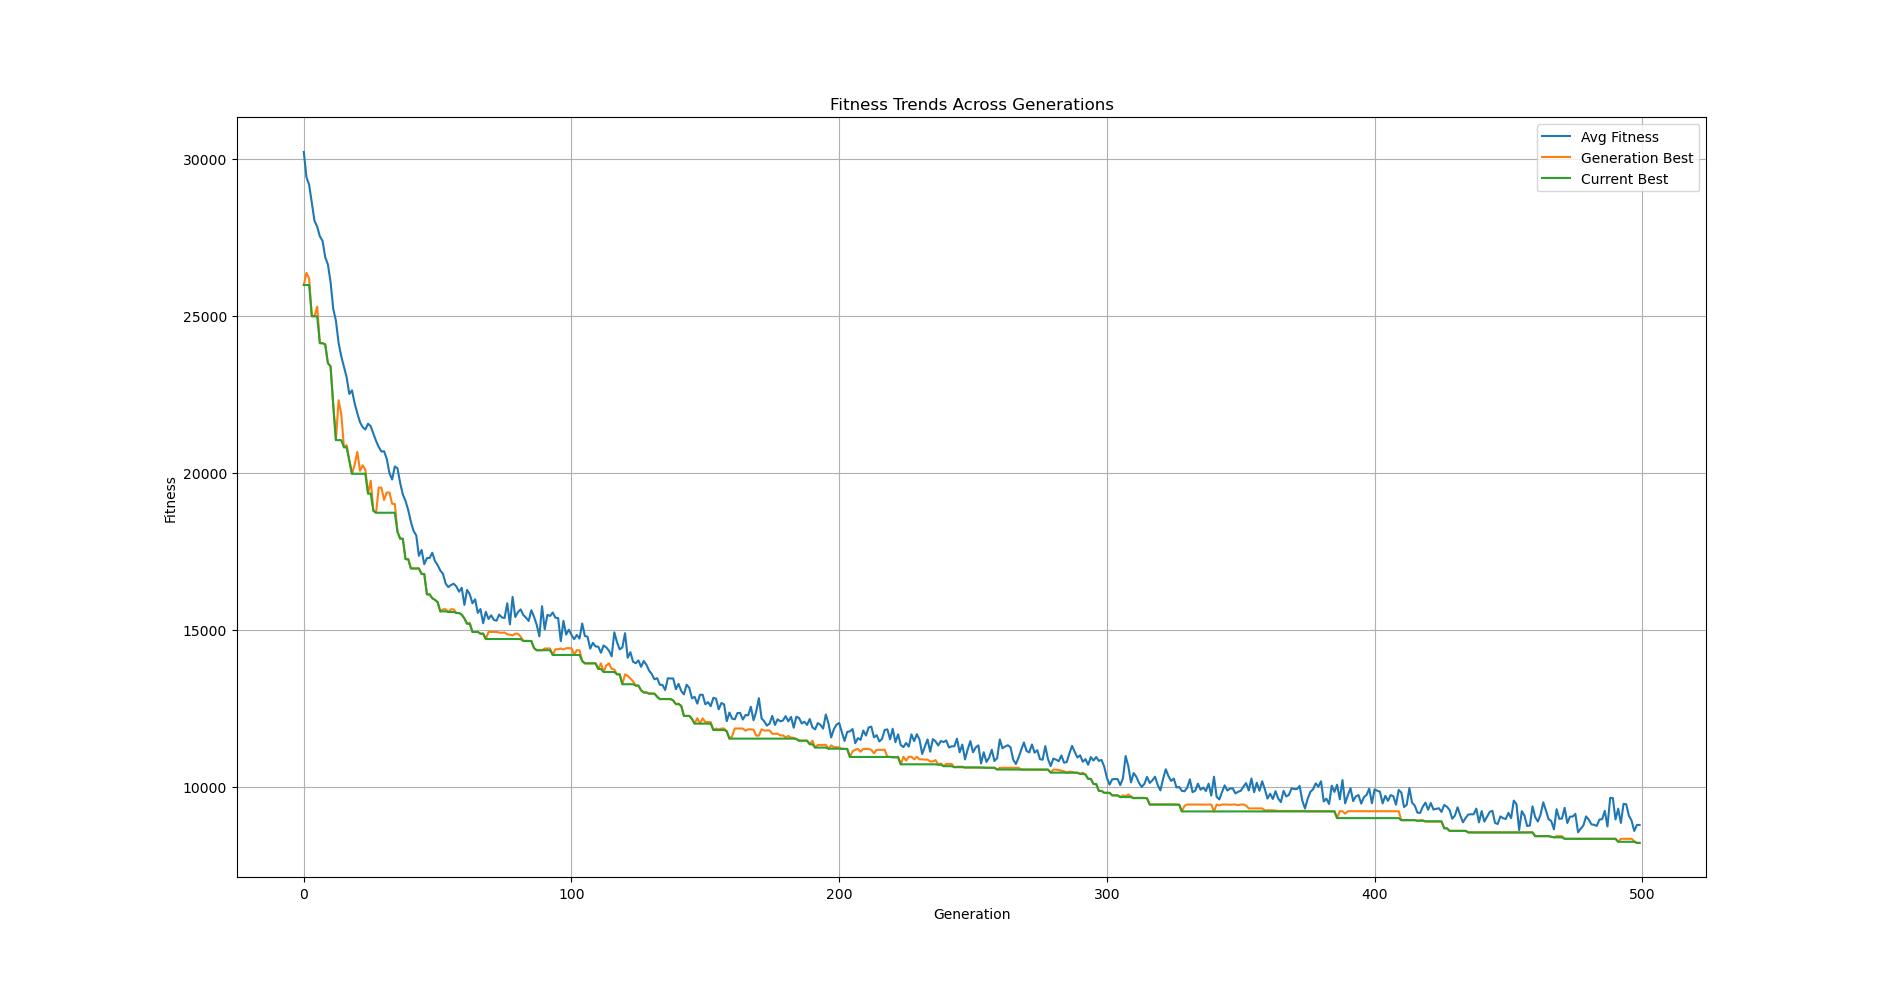
\includegraphics[width=\textwidth]{./images/berlin52_defaults_pmxonly.png}
\caption{Fitness achieved with PMX crossover alone on \texttt{berling52.tsp} using the default parameters}
\end{figure}

As can be seen from the above diagrams, the OX operator seemed to be destroying learned good paths as the average fitness started to fluctuate wildly and improve very little after a short period of learning.
With PMX crossover only however, the learning curve was much closer to the expected asymptotic curve, with average fitness steadily falling over generations and slowly bottoming-out.
Interestingly, even on the small \verb|berlin52.tsp| dataset, the effect of the relatively more simply OX operator being used could be seen, as the PMX+OX run took about half a second less.
This may be partially due to the fact that the PMX+OX crossover gave up after 452 generations while PMX-only ran the full 500 generations but the small difference in number of generations alone doesn't fully account for this discrepancy.

\subsubsection{Mutation}
Mutation was implemented much in the same way as crossover, with a generalised \mintinline{python}{mutate(offspring, mutation_rate)} function which accepted a list of the offspring produced via crossover and returned that list with mutations applied.
This function also randomly alternated between two mutation operators: Reverse Sequence Mutation (RSM) and Partial Shuffle Mutation (PSM).
I took the algorithmic steps for these functions from a paper titled \citetitle{adboun}.\supercite{adboun}
\\\\
The RSM operator was implemented as follows:
first, two random start and end indices are selected from the tour to delimit the sub-sequence to be reversed.
If the start index occurs after the end, they are swapped.
Then, that sub-sequence is simply reversed and the tour returned.
This simple operator maintains city adjacency while inserting some variance into a tour, thus increasing diversity without sacrificing what has already been learned by the algorithm.
\\\\
The PSM operator was implemented as follows:
again, two random start and end indices are selected as in the RSM operator, and the sub-sequence delimited by these indices is randomly shuffled by Python's \mintinline{python}{random.shuffle()} function, and the tour is returned.
This operator is both computationally and functionally more complex than RSM, and introduces a great deal more variability and helps to avoid early convergence.

\subsection{Grid Search}
The entire genetic algorithm logic was implemented in a function named \texttt{evolve(graph, adjacency\_matrix, population\_size, num\_generations, give\_up\_after, selection\_proportion, crossover\_rate, mutation\_rate, output\_file)}
which allowed for it to be called with different parameters for testing purposes.
A function named \texttt{grid\_search(graph, adjacency\_matrix, num\_generations, give\_up\_after, selection\_proportion, population\_sizes, crossover\_rates, mutation\_rates)} was then implemented which accepts lists of population sizes, crossover rates, \& mutation rates instead of single values, and iterates over each possible combination to find the combination which produces the best results.
I decided to hard-code these list values into the \mintinline{python}{main()} function of the script, as passing several lists of options to the program via command-line flags proved far more cumbersome than simply editing the file.
If the flag \texttt{--grid-search} is passed to the script, it runs the \texttt{grid\_search()} function instead of just the \texttt{evolve()} function.

\subsection{Plotting}
As previously mentioned, I chose to implement the plotting of fitness over generations in its own script named \verb|plots.py| which accepts a single TSV file as an argument and plots the fitness.
I also wrote a script called \verb|map.py| that plots a given hard-coded tour around cities defined in a TSP file, each located at their relative co-ordinates for visualisation purposes.
However, I wrote this script in a very quick and dirty way so it accepts no command-line arguments and must be edited to run on different files or with different tours.

\section{Experimental Results \& Analysis}
\subsection{\texttt{berlin52.tsp}}
I ran a grid search for \verb|berlin52.tsp| using \texttt{population\_sizes = [50, 100, 200, 300, 500]}, \texttt{crossover\_rates = [0.6, 0.7, 0.8, 0.9, 1]}, and \texttt{mutation\_rates = [0.01, 0.05, 0.1, 0.15, 0.2]}, which I felt gave a reasonable range of possible combinations for the dataset without taking prohibitively long to run.
I ran the grid search a few times to weed out very lucky or unlucky runs:
the best solution found with the grid search was as follows, but I struggled to replicate it:
\begin{itemize}
    \item   Best solution: \texttt{[33, 43, 10, 9, 8, 41, 19, 45, 3, 17, 7, 2, 42, 21, 31, 18, 22, 1, 32, 49, 39, 36, 35, 34, 44, 50, 20, 23, 30, 29, 16, 46, 48, 37, 40, 38, 24, 5, 15, 6, 4, 25, 12, 28, 27, 26, 47, 14, 13, 52, 11, 51]}.
    \item   Best solution fitness: 7842.999708659402.
    \item   Population size: 300.
    \item   Crossover rate: 0.8.
    \item   Mutation rate: 0.1.
    \item Time taken: 5.580028772354126 seconds.
\end{itemize}

\begin{figure}[H]
    \centering
    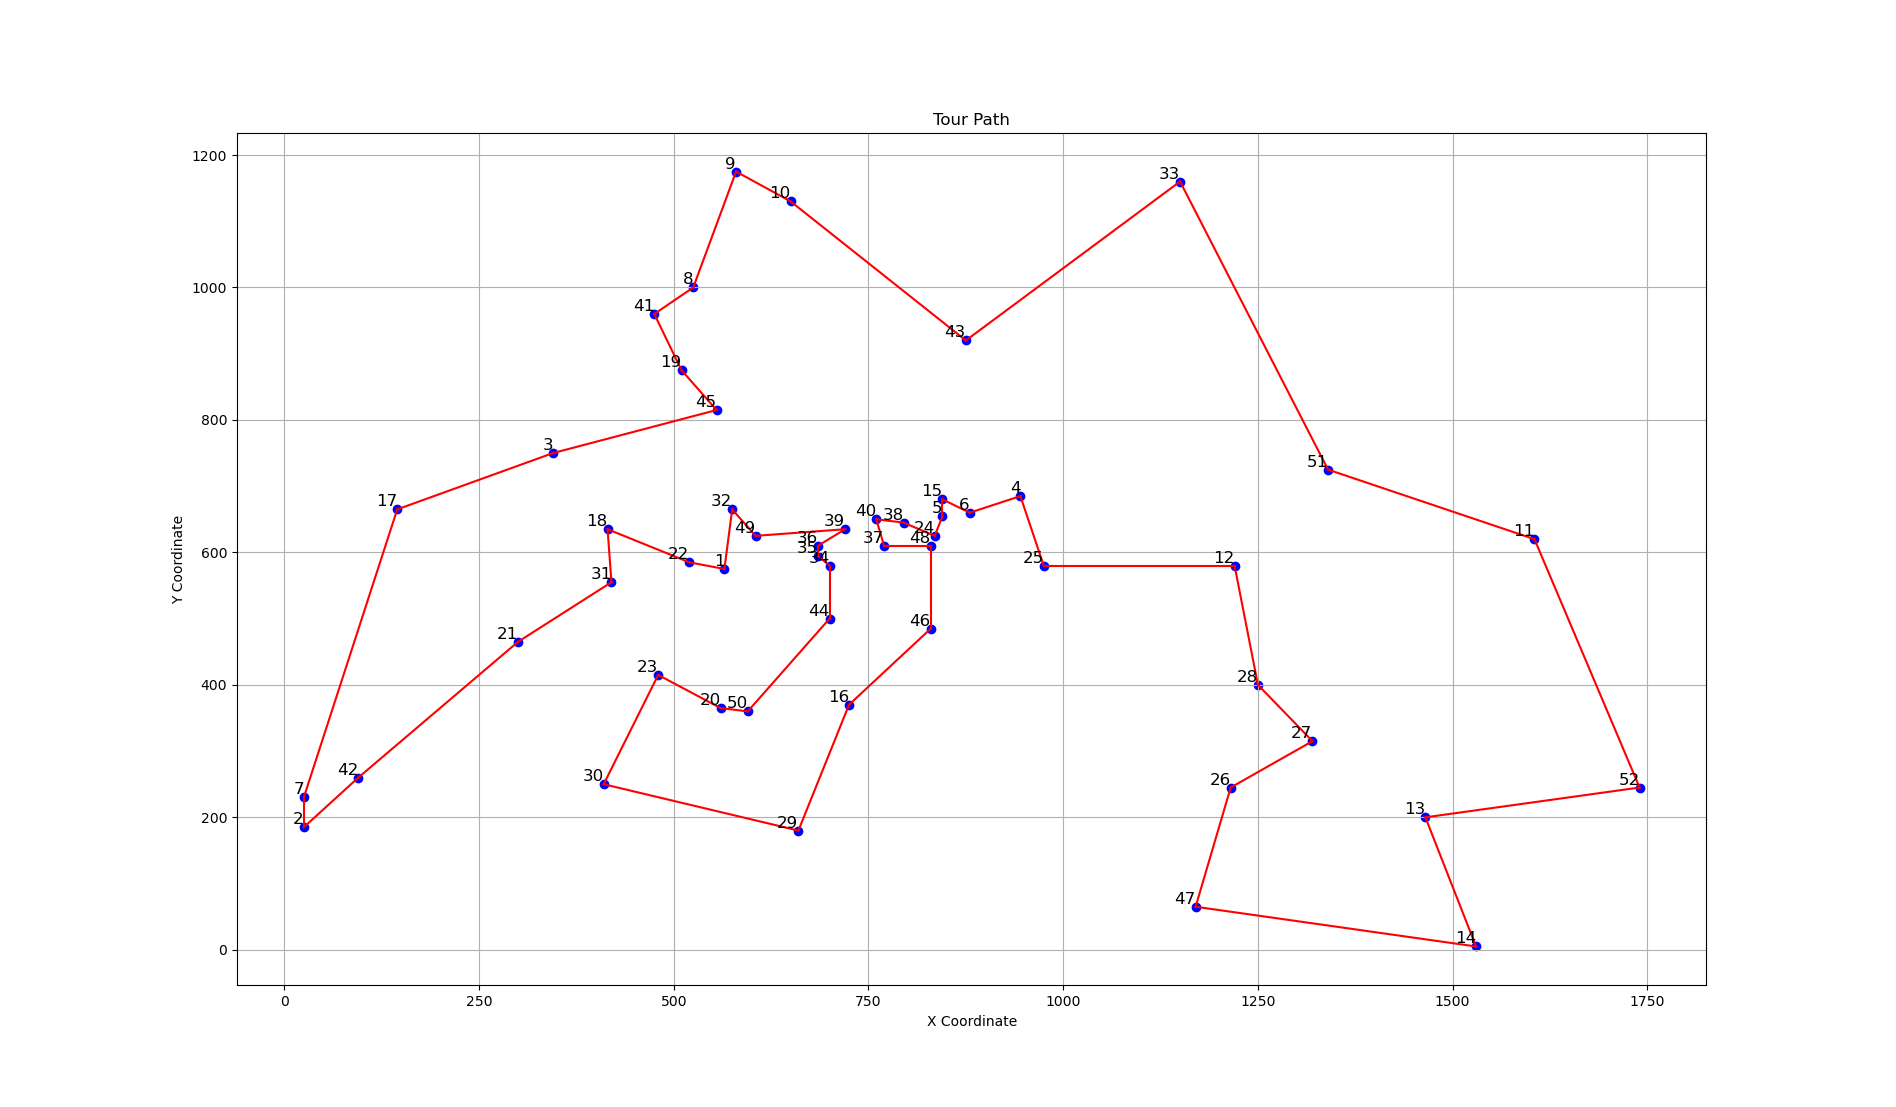
\includegraphics[width=\textwidth]{./images/berlin52besttour.png}
    \caption{Path taken by the best solution found for \texttt{berlin52.tsp} (fitness: 7842.999708659402)}
\end{figure}

However, in general, the best fitness found tended to be in the low 8000s with those parameters.
A more representative run yielded the following results:
\begin{itemize}
    \item   Best solution found: \texttt{[45, 19, 41, 8, 9, 10, 33, 43, 15, 38, 40, 37, 48, 24, 5, 6, 4, 25, 12, 51, 11, 52, 14, 13, 27, 28, 26, 47, 29, 50, 20, 23, 30, 2, 7, 42, 21, 17, 3, 18, 31, 22, 1, 44, 16, 46, 34, 39, 36, 35, 49, 32]}.
    \item   Fitness of best solution: 8012.642652424814.
    \item   Best solution found in generation: 386.
    \item   Time taken: 4.9562294483184814 seconds.
\end{itemize}

\begin{figure}[H]
    \centering
    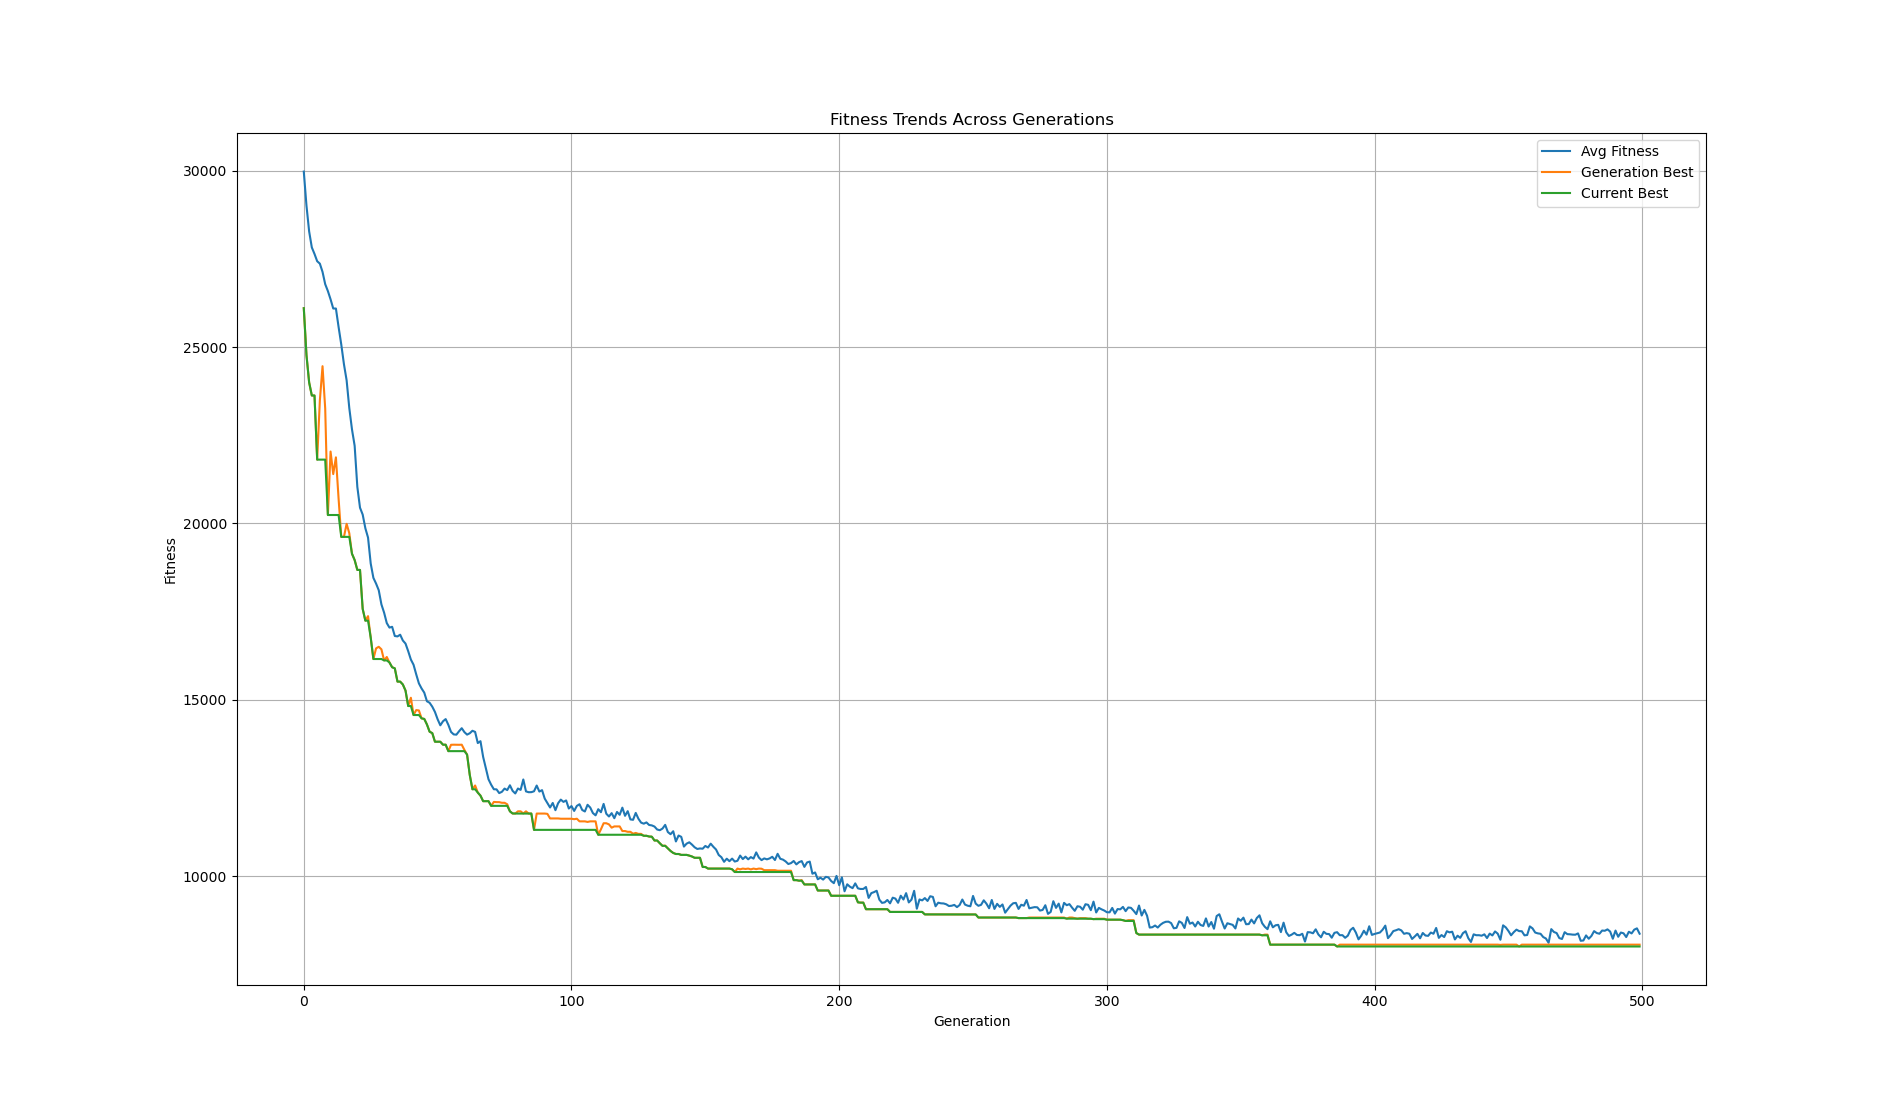
\includegraphics[width=\textwidth]{./images/berlin52rep.png}
    \caption{Fitness over generations for \texttt{berlin52.tsp} (best fitness: 8012.642652424814)}
\end{figure}

The algorithm behaved largely as expected, with improvements in fitness bottoming out towards the end of the run.
The best known fitness for the \texttt{berlin52.tsp} dataset is 7542, and since the average fitness of random permutation can be seen in the above diagram to be around 30,000, I am quite happy with this result.
The best solution we found ended up being only 300 out from the best possible solution.

\subsection{\texttt{kroA100.tsp}}
I noticed that the graph of the results wasn't bottoming-out as expected and that the algorithm wasn't giving up but was just reaching the end of its allotted number of generations, which indicated to me that the number of generations specified was restricting the algorithm.
To remedy this, I set the number of generations arbitrarily high, and relied on the give-up-after value to terminate the program when improvements were no longer being made.
I also found that using a much larger population size (1000) gave good, albeit slow results.
A run with these values yielded the following results:
\begin{itemize}
    \item   Best solution found: \texttt{[81, 25, 87, 51, 61, 58, 93, 28, 67, 89, 42, 31, 80, 56, 97, 75, 19, 4, 65, 26, 66, 70, 22, 94, 16, 88, 18, 24, 38, 99, 36, 59, 74, 21, 72, 10, 84, 79, 53, 90, 49, 6, 63, 92, 8, 1, 47, 11, 17, 15, 32, 45, 91, 98, 23, 60, 62, 35, 86, 27, 20, 77, 57, 9, 7, 12, 55, 83, 34, 29, 46, 43, 3, 14, 71, 41, 100, 48, 52, 78, 96, 13, 76, 33, 37, 5, 39, 30, 85, 68, 73, 50, 44, 82, 95, 2, 54, 40, 64, 69]}.
    \item   Fitness of best solution: 23931.38351530833.
    \item   Best solution found in generation: 1303.
    \item   Time taken: 154.4610664844513.
\end{itemize}

\begin{figure}[H]
    \centering
    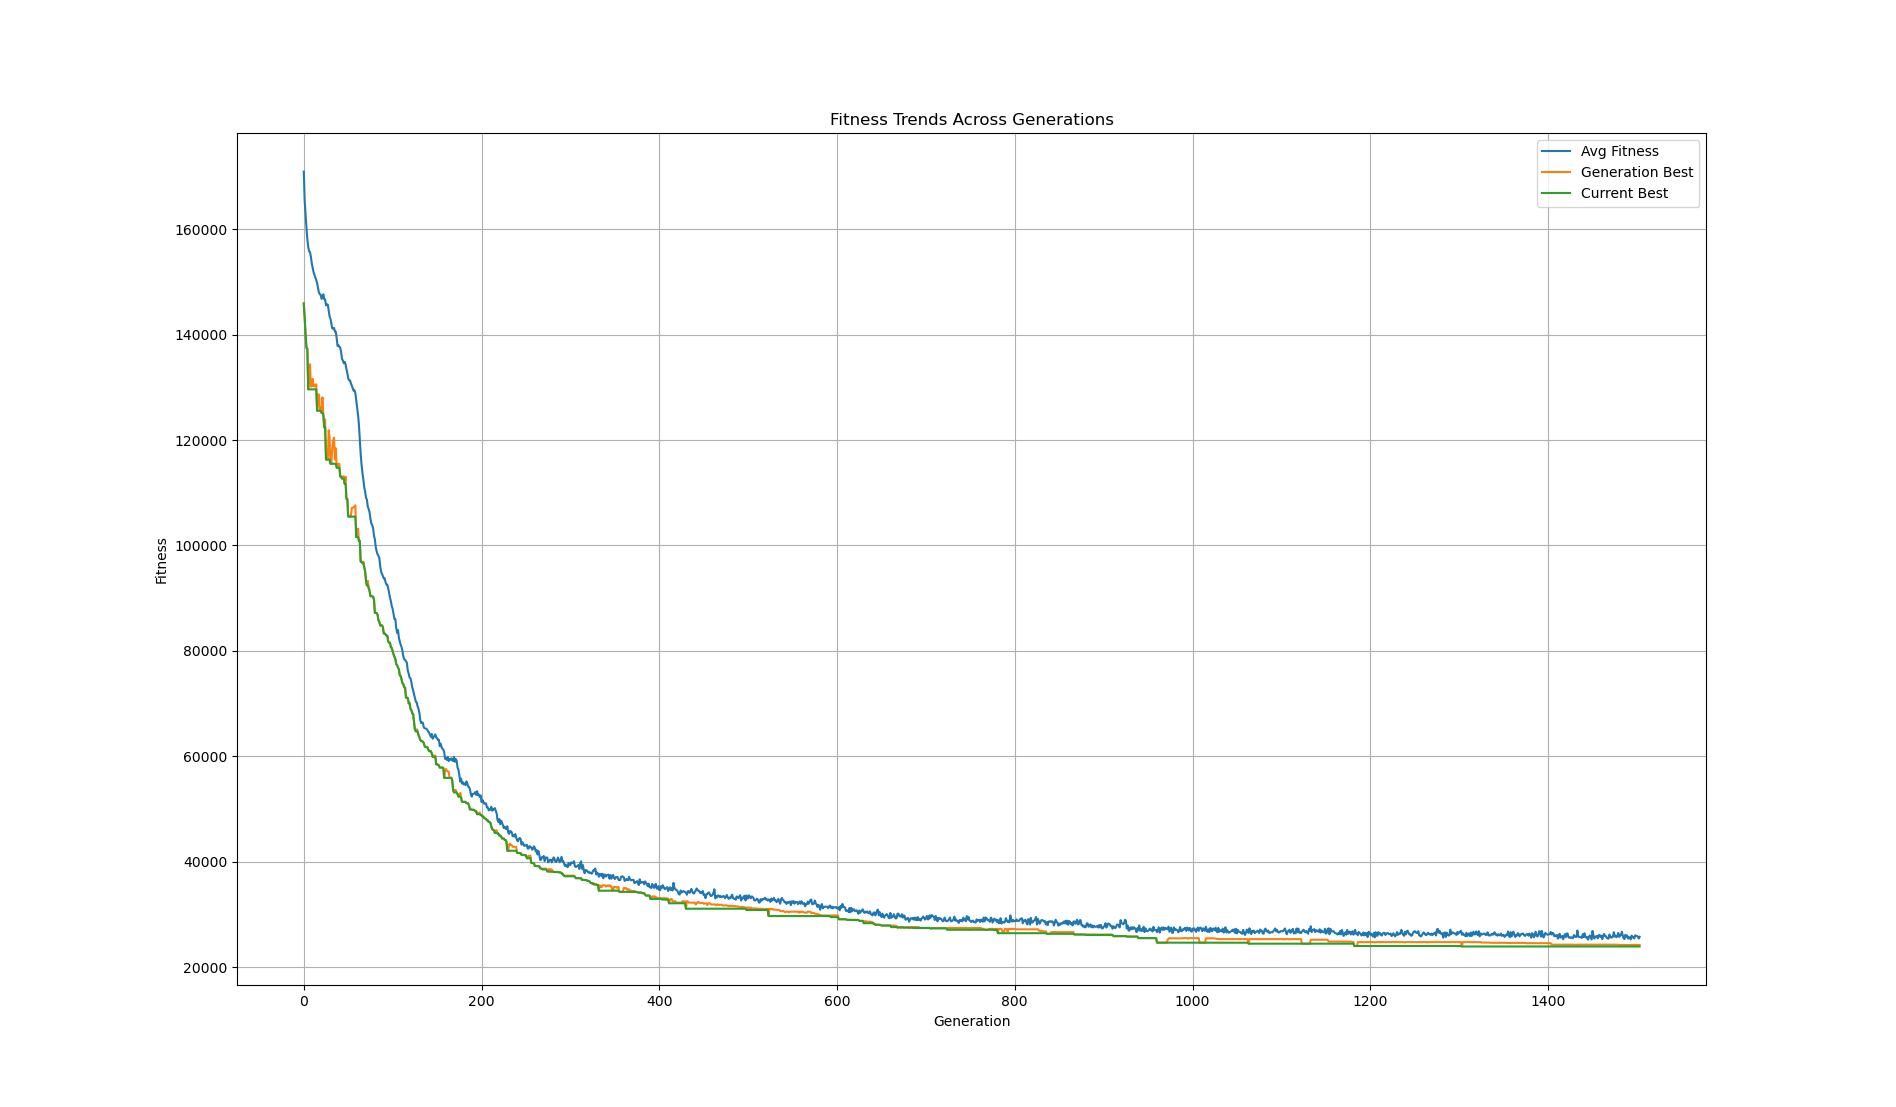
\includegraphics[width=\textwidth]{./images/betterkroaplot.png}
    \caption{Fitness over generations for \texttt{kroA100.tsp} (best fitness: 23931.38351530833)}
\end{figure}

\begin{figure}[H]
    \centering
    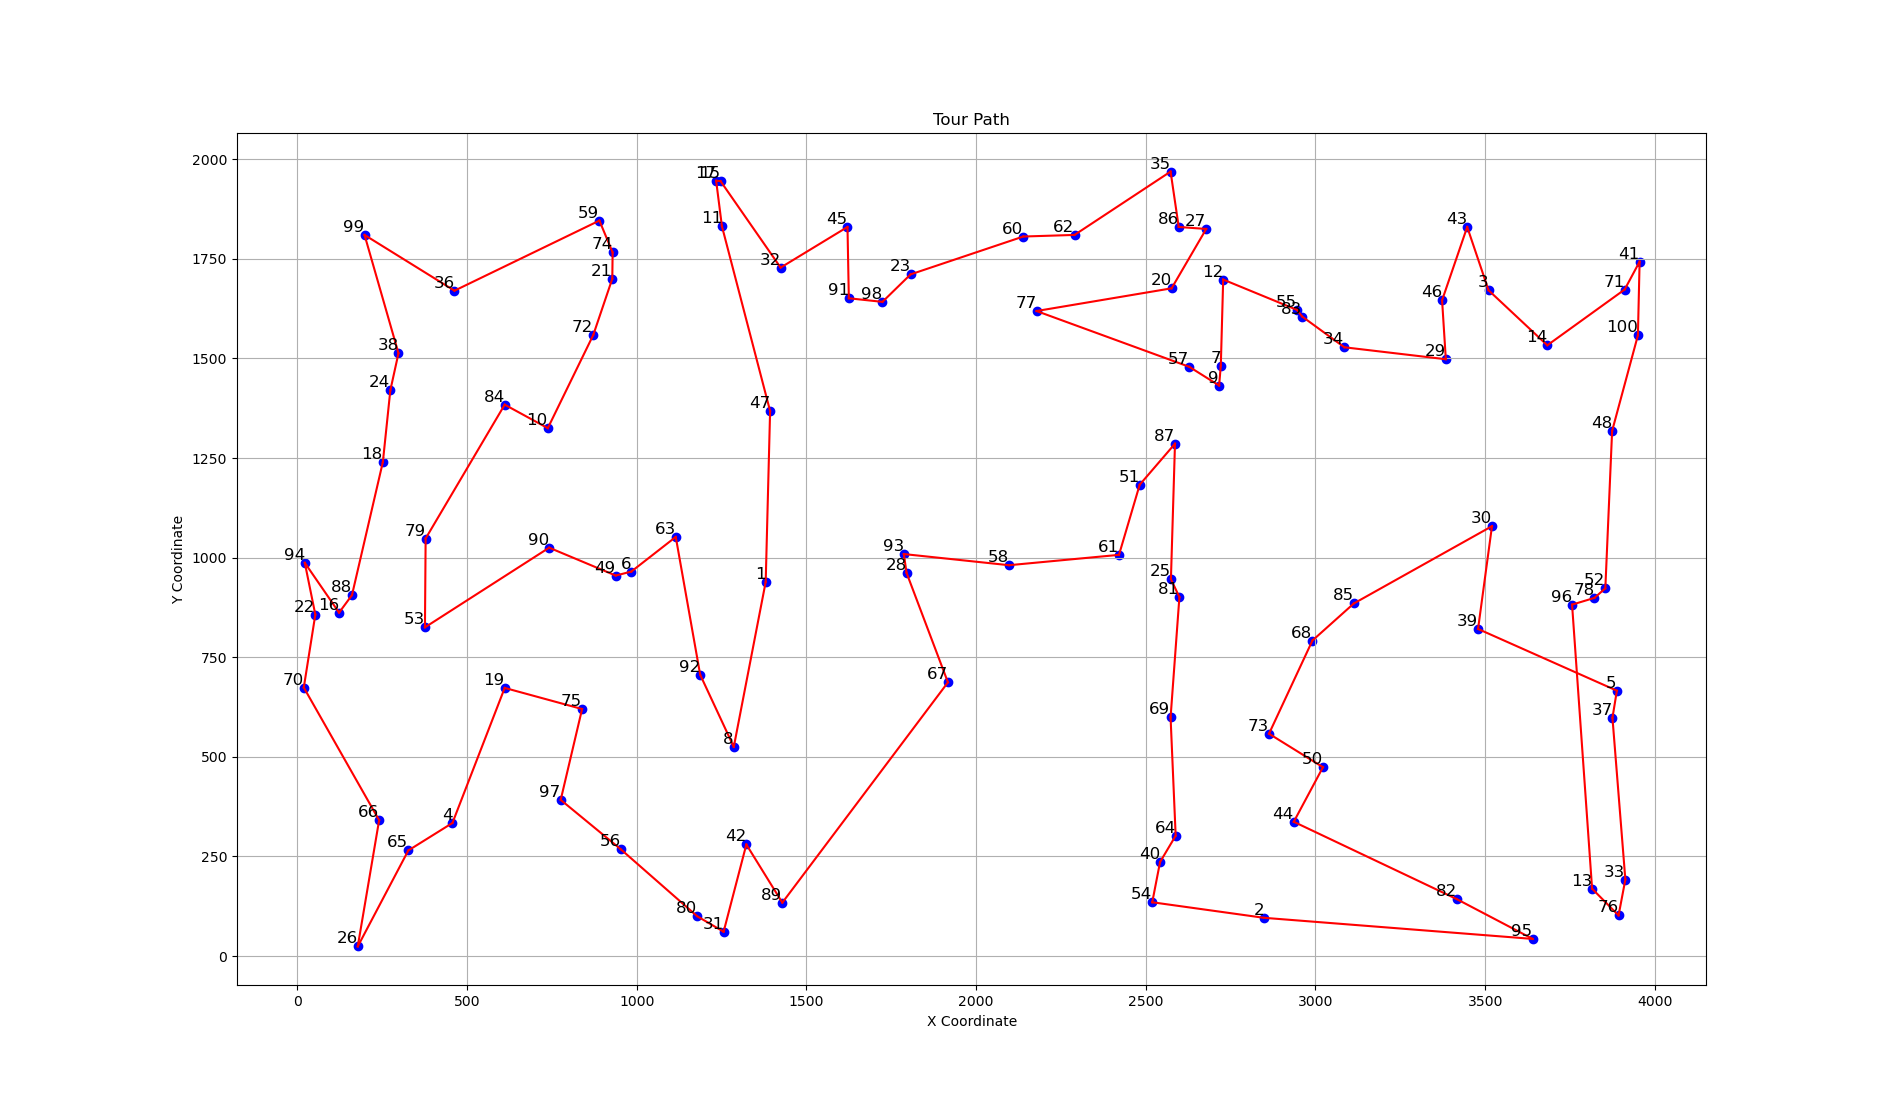
\includegraphics[width=\textwidth]{./images/beterkroapath.png}
    \caption{Path taken by the best solution found for \texttt{kroA100.tsp}}
\end{figure}

It is worth noting here that as the population size and number of generations are increased, it gets closer and closer to just being a really bad brute-force search and this could be argued to be part of the reason for the greater success with higher values.
However, I would argue that this does not account for the results seen in the fitness-over-generations plot, as the average fitness is steadily decreasing right up until the end which can only happen if the algorithm is indeed learning.
The best known solution for this problem has a fitness of 21,282 and the best result I achieved was 23,931 which is just 2,649 or so out, which I am happy with as a randomly generated solution has an average fitness in excess of 160,000 for this dataset.

\subsection{\texttt{pr1002.tsp}}
I didn't conduct a grid search on the \texttt{pr1002.tsp} dataset because it took prohibitively long to run:
I attempted once but it was showing no signs of stopping hours later so I gave up.
I performed a single run with a population size of 300, a crossover rate of 0.8, and a mutation rate of 0.1 for 5000 generations.
Originally, I had chosen the number 5000 as an arbitrarily large number that would never be reached, as the algorithm would give up after 200 generations of no change; 
however, the program kept running for the entire 5000 generations, taking just over 3 hours to complete.
The results were quite interesting:

\begin{figure}[H]
    \centering
    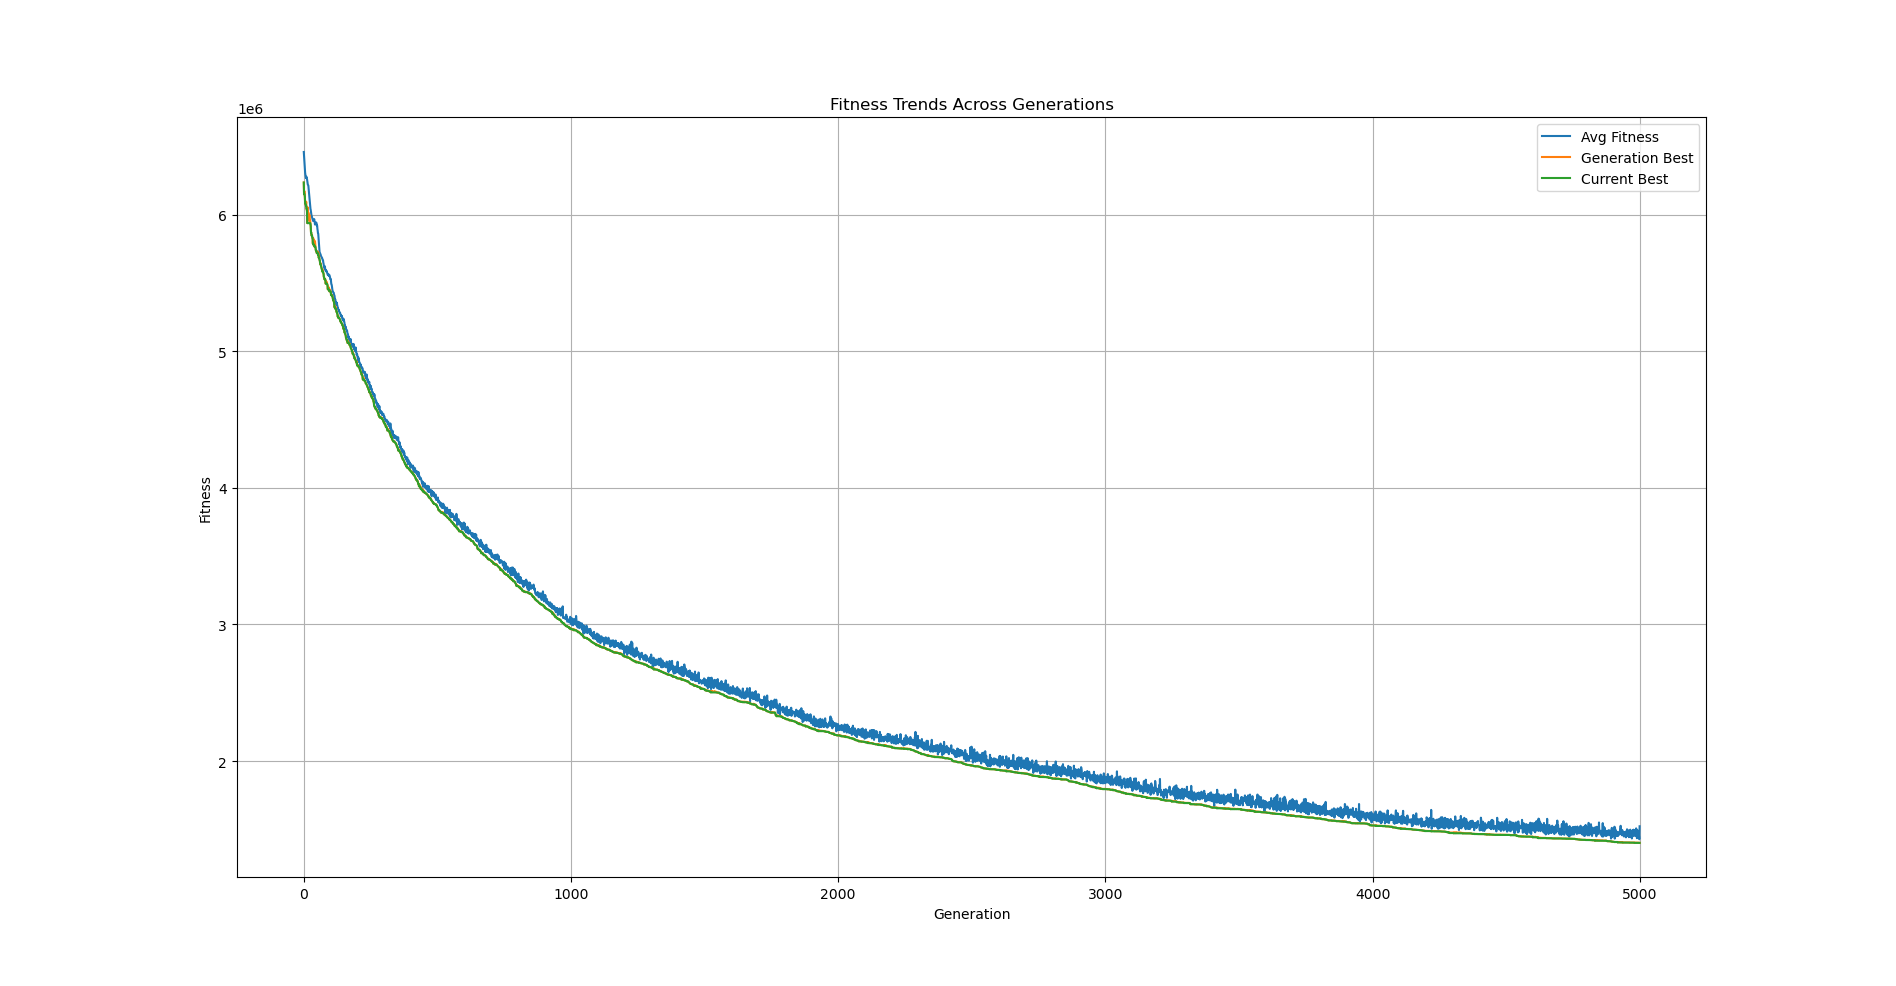
\includegraphics[width=\textwidth]{./images/pr1002fitness.png}
    \caption{Fitness over generations for \texttt{pr1002} (best fitness: 1,401,503.549568915)}
\end{figure}

The best fitness in question was found in the 4979\textsuperscript{th} generation: clearly, the  graph has not yet flattened out even after 5000 generations which indicates that it was still learning and improving and was cut short.
The average fitness over the generations is also quite interesting: despite trending steadily downwards, it fluctuates greatly within a narrow range.
This suggests to me that there was always a great deal of diversity within the solution pool, which is probably in no small part due to the fact that the dataset had so many points that a great deal of permutations were possible.
I would be inclined to think that the number of generations required to converge on a solution for a dataset would scale with the number of possible paths through the network, $N!$, and therefore I would guess that this particular dataset would require thousands of more iterations before converging on a good solution.
\\\\
The best known fitness for this dataset is 259,045: clearly our result was quite a bit out, but this is more as a result of the evolution process being cut short before convergence.
For the sake of completeness, I'll include the best path found during that search, but anyone can tell just by looking at it that it is very far from the shortest possible path:

\begin{figure}[H]
    \centering
    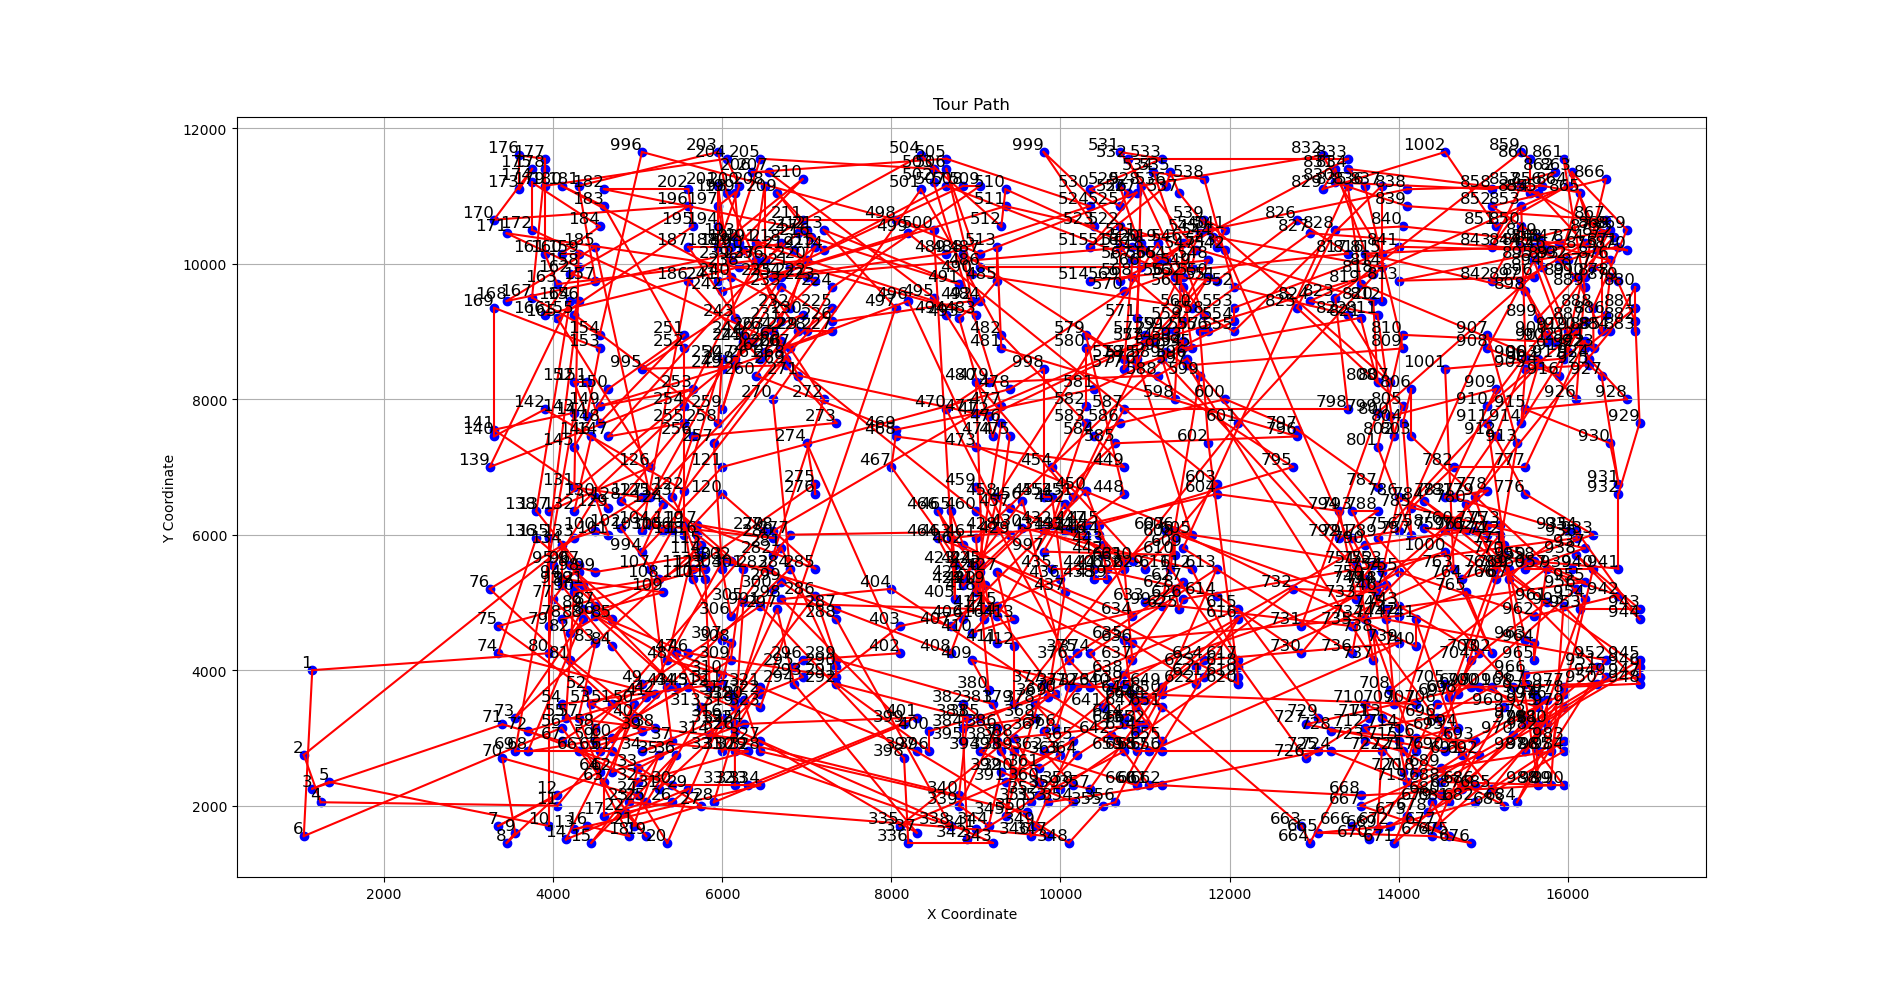
\includegraphics[width=0.75\textwidth]{./images/pr1002path.png}
    \caption{Path taken by the best solution found for \texttt{pr1002.tsp}}
\end{figure}



\section{Potential Improvements}
There are a great deal of potential improvements that could be made to my implementation, the majority of which I unfortunately did not have time to implement.
These include:
\begin{itemize}
    \item   Writing it in a different programming language: while I previously referred to how parsing the input TSP files would be much easier using Perl due to its convenient \& powerful regex, if I were to write this program again I would probably opt for C.
            When I set out to write this program I didn't really know what I was in for, so I chose Python because it would allow me a great deal of flexibility and because it would be relatively fast to write.
            However, I don't really make great use of any Python-specific features and I repeatedly found myself attempting to strip back the layers of abstraction built into Python to find the big-O complexity of certain operations.
            For example, I didn't use any fancy data structure to represent the graph, just an adjacency matrix using arrays.
            Furthermore, there are a great number of ``gotchas'' that one can easily fall into when writing performance-critical Python code, such as some function that will be run on every possible tour in every generation, where time-step complexity multiplies fast.
            For example, a simple line of code to find the index of the lowest fitness in a list of fitnesses such as \mintinline{python}{best_index = fitnesses.index(min(fitnesses))} which appears simple \& elegant has a big-O complexity of $O(2n)$ because the \mintinline{python}{min()} function searches the entire unsorted list for the minimum value and the \mintinline{python}{list.index()} function also searches the entire unsorted list for the value given.
            Thus, if you were running this line of code every generation, the program would quickly become very inefficient, and there are so many ``gotchas'' like this which I came across when writing my code.

    \item   The initial population could be created by some heuristic-based mechanism rather than by random permutations, which could potentially speed up convergence.

    \item   It's not unlikely that the same tours were evolved independently on multiple occasions during a single run of the genetic algorithm, and the fitness for these independently-evolved twins would be re-calculated every time they appeared. 
            Instead, it would possibly be more efficient to hash each tour and store its fitness in a hash table instead of re-calculating it every time, although this is dependent on how often we expect the same tour to appear in each run.

    \item   A greater number of mutation and crossover operators could be implemented and tested to find optimal ones.

    \item   There was no distinction between different stages of the search in my implementation;
            adapting behaviour based on the stage of the search could improve performance.
            For example, as the average fitness of each generation starts to stagnate and improvement grinds to a halt, the algorithm could become increasingly reckless, increasing the mutation rate to increase diversity and attempt to burst out of the potential local maxima in which it was getting stuck.
            Different crossover and mutation operators could be employed at different stages of the search.

    \item   Grid search with more parameters: many parameters went relatively untuned throughout this assignment, such as the number of generations, the probabilities of different crossover \& mutation operators, and the selection proportion.

    \item   I potentially lost out on the benefits of Monte Carlo selection by not taking the time to fine-tune a fitness-based weighting scheme for the probabilistic selection.
            More selection algorithms could have been tried \& tested as well, such as elitism.

    \item   Some kind of parallelisation could have been implemented to speed up the execution time.

    \item   Some kind of technique like simulated annealing could have been used to try and find the global optimum for the problem.

\end{itemize}

\nocite{*}
\printbibliography

\end{document}
